\documentclass[11pt,a4paper]{article}

\usepackage[margin=1in]{geometry}
\usepackage{mathptmx}
\usepackage{amsmath}
\usepackage{amssymb}
\usepackage{amsthm}
\usepackage{braket}
\usepackage{tikz}
\usetikzlibrary{shapes.geometric}
\usepackage{quantikz}
\usepackage{enumitem}
\usepackage{hyperref}
\usepackage{xcolor}

\definecolor{circuitblue}{RGB}{40,80,160}

\hypersetup{
    colorlinks=true,
    linkcolor=circuitblue,
    urlcolor=circuitblue,
    citecolor=circuitblue
}

\theoremstyle{definition}
\newtheorem{definition}{Definition}[section]
\newtheorem{example}{Example}[section]
\newtheorem{theorem}{Theorem}[section]

\theoremstyle{remark}
\newtheorem*{intuition}{Intuition}
\newtheorem*{keypoint}{Key Point}

\pagestyle{plain}

\setlength{\parindent}{0pt}
\setlength{\parskip}{6pt}

\begin{document}

\begin{center}
    {\LARGE \textbf{Barren Plateaus and Trainability Issues}}\\[8pt]
    {\large QML}\\[12pt]
    \hrule
\end{center}

\vspace{12pt}
\tableofcontents
\newpage

%% ========================================================
\section{Overview}
%% ========================================================

this is arguably the most important lecture in the entire course. barren plateaus r the central obstacle to scaling variational quantum algorithms, and understanding them is essential for anyone who wants to design practical quantum ML models.

the basic problem: when u train a parameterized quantum circuit by gradient descent, the gradients can vanish \emph{exponentially} in the number of qubits. not polynomially --- exponentially. this means that for a 100-qubit circuit, the gradient might be $\sim 2^{-100}$, which is indistinguishable from zero with any reasonable number of measurement shots.

this isnt just a theoretical concern --- its the main reason why scaling VQAs to useful problem sizes has been so difficult. in this lecture, well understand exactly why barren plateaus happen, when they occur, and wt we can do about them.

the good news: we now understand barren plateaus well enough to avoid them in many cases. the bad news: avoiding them often means restricting the model in ways that might limit its power. this tension between trainability and expressiveness is the central challenge of variational QML.

%% ========================================================
\section{What Is a Barren Plateau?}
%% ========================================================

\subsection{Formal Definition}

\begin{definition}[Barren Plateau]
a parameterized quantum circuit $U(\theta)$ with cost function $C(\theta)$ exhibits a \textbf{barren plateau} if the variance of the cost function partial derivatives vanishes exponentially with the number of qubits $n$:
\begin{equation}
    \text{Var}_\theta\left[\frac{\partial C}{\partial \theta_k}\right] \leq F(n) \in O\left(\frac{1}{b^n}\right)
\end{equation}
for some $b > 1$, where the variance is taken over random parameter initializations $\theta$.
\end{definition}

wt does this mean in practice? if the gradient variance is $O(2^{-n})$, then to estimate the gradient to precision $\epsilon$, u need:
\begin{equation}
    N_{\text{shots}} = O\left(\frac{\text{Var}[\partial_k C]}{\epsilon^2}\right) = O\left(\frac{1}{\epsilon^2 \cdot 2^n}\right)
\end{equation}
wait thats wrong --- u actually need \emph{more} shots when the signal is small. the number of measurements to distinguish the gradient from zero is:
\begin{equation}
    N_{\text{shots}} = O\left(\frac{1}{(\partial_k C)^2}\right) = O(2^n)
\end{equation}
bcs the gradient itself is typically $O(2^{-n/2})$ when the variance is $O(2^{-n})$.

\begin{intuition}
imagine trying to find the lowest point in a landscape thats almost perfectly flat, with tiny random bumps of height $\sim 2^{-n}$. u cant tell which direction is downhill bcs ur measurement noise is way larger than the actual slope. thats a barren plateau. the landscape isnt featureless --- it has structure --- but the structure is invisible to any polynomial-time optimization procedure.
\end{intuition}

\subsection{Why This Is Devastating}

the exponential scaling is wt makes barren plateaus qualitatively different from the vanishing gradient problem in classical deep learning. in classical NNs:
\begin{itemize}
    \item gradients vanish \emph{polynomially} with depth (for vanilla networks without skip connections)
    \item solutions exist: residual connections, batch normalization, careful initialization
    \item these solutions work well in practice
\end{itemize}

in quantum circuits:
\begin{itemize}
    \item gradients vanish \emph{exponentially} with width (number of qubits)
    \item no analog of residual connections (unitarity prevents additive shortcuts)
    \item the problem is fundamental, not just a practical inconvenience
\end{itemize}

\begin{keypoint}
barren plateaus r not just ``quantum vanishing gradients.'' the exponential scaling makes them qualitatively worse. in a classical network with vanishing gradients, u can often still make progress (slowly). in a barren plateau, the gradient is literally smaller than ur measurement precision for any practical number of shots. ur optimizer is effectively taking random walks.
\end{keypoint}

%% ========================================================
\section{The Original Result: McClean et al. 2018}
%% ========================================================

the foundational paper by mcclean, boixo, smelyanskiy, napp, and babbush (2018) established that random parameterized quantum circuits generically exhibit barren plateaus.

\subsection{Setup}

consider a parameterized circuit:
\begin{equation}
    U(\theta) = U_L(\theta_L) \cdots U_2(\theta_2) \cdot U_1(\theta_1)
\end{equation}
and a cost function:
\begin{equation}
    C(\theta) = \bra{0} U^\dagger(\theta) \, O \, U(\theta) \ket{0}
\end{equation}
where $O$ is some observable (hermitian operator).

the partial derivative with respect to parameter $\theta_k$ (assuming it appears in gate $U_k = e^{-i\theta_k P_k/2}$ for some pauli $P_k$) is:
\begin{equation}
    \frac{\partial C}{\partial \theta_k} = \frac{i}{2} \bra{0} U^\dagger(\theta) \, [U_{k+}^\dagger O U_{k+} - U_{k-}^\dagger O U_{k-}] \, U(\theta) \ket{0}
\end{equation}
where we use the fact that the parameter shift rule gives:
\begin{equation}
    \frac{\partial C}{\partial \theta_k} = \frac{1}{2}\Big[C(\theta_k + \pi/2) - C(\theta_k - \pi/2)\Big]
\end{equation}

\subsection{The Key Theorem}

\begin{theorem}[McClean et al. 2018 --- Barren Plateau Theorem]
let $U(\theta) = U_L \cdots U_1$ be a parameterized quantum circuit on $n$ qubits. suppose the gates $\{U_l\}$ form a 2-design (i.e., the distribution of unitaries matches the Haar measure up to the second moment). then for any observable $O$ and any parameter $\theta_k$:
\begin{equation}
    \mathbb{E}_\theta\left[\frac{\partial C}{\partial \theta_k}\right] = 0
\end{equation}
and
\begin{equation}
    \text{Var}_\theta\left[\frac{\partial C}{\partial \theta_k}\right] \leq \frac{2 \, \text{Tr}(O^2)}{2^{2n} - 1}
\end{equation}
which is $O(2^{-n})$ for any observable with polynomial $\text{Tr}(O^2)$.
\end{theorem}

\subsection{Proof Sketch}

the proof uses the theory of unitary $t$-designs and haar integration. here r the key steps:

\textbf{step 1: decompose the circuit.} write $U(\theta) = U_R \cdot V_k(\theta_k) \cdot U_L$ where $U_L$ contains all gates before gate $k$, $V_k$ is the gate containing $\theta_k$, and $U_R$ contains all gates after.

\textbf{step 2: compute the gradient.}
\begin{equation}
    \partial_k C = \frac{i}{2} \text{Tr}\Big[O \, U_R V_k' U_L \ket{0}\bra{0} U_L^\dagger V_k^\dagger U_R^\dagger\Big]
\end{equation}
where $V_k' = [P_k, V_k]/2$ involves the commutator with the generator.

\textbf{step 3: average over $U_L$ using 2-design property.} when $U_L$ forms a 2-design, we can use the haar integral formula:
\begin{equation}
    \int dU \; U \rho U^\dagger \otimes U \sigma U^\dagger = \frac{\text{Tr}(\rho)\text{Tr}(\sigma) + \text{Tr}(\rho\sigma)}{d(d+1)} (\mathbb{I} + \text{SWAP}) + \cdots
\end{equation}
where $d = 2^n$.

\textbf{step 4: average over $U_R$ similarly.} the combination of averaging over both $U_L$ and $U_R$ squeezes out all the structure from the circuit, leaving only dimension-dependent factors.

\textbf{step 5: bound the variance.} after integrating, the variance picks up a factor of $1/d^2 = 1/4^n$:
\begin{equation}
    \text{Var}[\partial_k C] = O\left(\frac{\|O\|^2_F}{4^n}\right)
\end{equation}
where $\|O\|_F^2 = \text{Tr}(O^2)$.

\begin{intuition}
the proof boils down to: if ur circuit is expressive enough to look like a random unitary, then the cost landscape becomes flat bcs a random unitary ``scrambles'' all information. the observable $O$ gets diluted across the entire $2^n$-dimensional hilbert space, and the gradient signal drowns in the exponentially large space.
\end{intuition}

\subsection{The 2-Design Condition}

a key assumption is that the circuit forms a 2-design. when does this happen?

\begin{definition}[Unitary 2-Design]
an ensemble of unitaries $\{U_i\}$ forms a 2-design if:
\[
\mathbb{E}_i\left[U_i^{\otimes 2} \rho (U_i^\dagger)^{\otimes 2}\right] = \int_{\text{Haar}} U^{\otimes 2} \rho (U^\dagger)^{\otimes 2} \, dU
\]
for all operators $\rho$ on $(\mathbb{C}^d)^{\otimes 2}$.
\end{definition}

in practice, many common ansatz architectures converge to 2-designs quickly:
\begin{itemize}
    \item random circuits with CNOT + single-qubit rotations: becomes 2-design in $O(n)$ depth
    \item hardware-efficient ansatz (HEA): typically becomes 2-design within a few layers
    \item the more expressive ur circuit, the faster it converges to 2-design, and the worse the barren plateau
\end{itemize}

\begin{keypoint}
this is the fundamental irony: \emph{more expressiveness leads to worse trainability}. if ur circuit can express everything, it can learn nothing (efficiently). this is the expressibility-trainability tradeoff, and its the most important concept in this lecture.
\end{keypoint}

%% ========================================================
\section{Cost Function Dependent Barren Plateaus}
%% ========================================================

cerezo, sone, volkoff, cincio, and coles (2021) showed that barren plateaus depend critically on the cost function structure, not just the circuit.

\subsection{Global vs Local Cost Functions}

\begin{definition}[Global Cost Function]
a cost function $C = \text{Tr}[O \rho(\theta)]$ is \textbf{global} if the observable $O$ acts non-trivially on all $n$ qubits. example: $O = \ket{\psi}\bra{\psi}$ for some target state $\ket{\psi}$ (state fidelity).
\end{definition}

\begin{definition}[Local Cost Function]
a cost function is \textbf{local} if $O = \frac{1}{n}\sum_{j=1}^{n} O_j$ where each $O_j$ acts on $O(1)$ qubits. example: $O = \frac{1}{n}\sum_j Z_j$ (average magnetization).
\end{definition}

\begin{theorem}[Cerezo et al. 2021 --- Cost-Dependent Barren Plateaus]
for a parameterized circuit forming a local 2-design:
\begin{enumerate}[label=(\roman*)]
    \item \textbf{global cost}: $\text{Var}[\partial_k C_G] \in O(2^{-n})$ --- exponential vanishing regardless of circuit depth
    \item \textbf{local cost}: $\text{Var}[\partial_k C_L] \in \Omega(2^{-2L})$ for a circuit of depth $L$ on $n$ qubits --- the gradient variance depends on the depth, not the width
\end{enumerate}
\end{theorem}

this is a huge deal. it says:

\begin{itemize}
    \item for global cost functions, ur screwed no matter wt --- barren plateaus kick in with system size $n$
    \item for local cost functions, u can avoid barren plateaus by keeping the circuit shallow! the gradient variance depends on depth $L$, so as long as $L \in O(\text{poly}(\log n))$, ur fine
\end{itemize}

\begin{example}
consider two cost functions for state preparation:
\begin{align}
    C_G &= 1 - |\bra{\psi_{\text{target}}} U(\theta) \ket{0}|^2 \quad \text{(global --- fidelity)} \\
    C_L &= 1 - \frac{1}{n} \sum_{j=1}^{n} \text{Tr}\big[\rho_j^{\text{target}} \, \rho_j(\theta)\big] \quad \text{(local --- reduced state fidelity)}
\end{align}
where $\rho_j$ is the reduced density matrix of qubit $j$. both cost functions vanish when $U(\theta)\ket{0} = \ket{\psi_{\text{target}}}$, but $C_L$ is much more trainable bcs it only involves local measurements.
\end{example}

\begin{intuition}
why does locality help? a local cost function only ``looks at'' a few qubits at a time. changing a parameter in the circuit has a local effect that propagates through the circuit. if the circuit is shallow, this effect hasnt been scrambled across all qubits yet, so the gradient retains a non-vanishing signal. a global cost function requires all qubits to cooperate simultaneously, which becomes exponentially unlikely as $n$ grows.
\end{intuition}

%% ========================================================
\section{Noise-Induced Barren Plateaus}
%% ========================================================

wang, larocca, czarnik, goyal, coles, and cerezo (2021) discovered smtg disturbing: hardware noise can \emph{independently} cause barren plateaus, even when the noiseless circuit would be trainable.

\subsection{The Result}

\begin{theorem}[Noise-Induced Barren Plateaus]
consider a parameterized circuit with local depolarizing noise after each gate, with noise rate $p$. for any cost function (even local ones), the gradient variance satisfies:
\begin{equation}
    \text{Var}[\partial_k C] \leq 2 \|O\|^2 \cdot q^{2L}
\end{equation}
where $q = 1 - p$ and $L$ is the circuit depth. when $L \geq O(1/p)$, the gradients vanish exponentially:
\begin{equation}
    \text{Var}[\partial_k C] \leq 2 \|O\|^2 \cdot e^{-2pL}
\end{equation}
\end{theorem}

this is independent of the cost function structure! even local cost functions --- which r safe from ``expressibility-induced'' barren plateaus --- suffer from noise-induced barren plateaus when the circuit is deep enough.

\begin{keypoint}
noise-induced barren plateaus set a hard depth limit on trainable circuits:
\begin{equation}
    L_{\text{max}} \sim \frac{1}{p}
\end{equation}
for typical NISQ error rates $p \sim 10^{-3}$ to $10^{-2}$, this means $L_{\text{max}} \sim 100$ to $1000$ layers. sounds like a lot, but remember that each ``layer'' might involve just one gate, so this limits circuit depth to $O(100\text{-}1000)$ total gates.
\end{keypoint}

\begin{intuition}
the mechanism is simple: noise pushes the quantum state toward the maximally mixed state $\mathbb{I}/2^n$. the maximally mixed state is a fixed point of any unitary, so all parameters become equally (un)important. the cost landscape flattens out bcs the state has lost all its quantum structure to decoherence.
\end{intuition}

\subsection{Implications}

this result creates a three-way tension:

\begin{enumerate}[label=\arabic*.]
    \item \textbf{expressibility} wants deep circuits (more parameters, more expressiveness)
    \item \textbf{trainability} wants shallow circuits (avoid barren plateaus)
    \item \textbf{noise tolerance} wants even shallower circuits (avoid noise-induced BPs)
\end{enumerate}

the viable region is the intersection of all three constraints:
\begin{equation}
    L_{\text{viable}} \leq \min\left(L_{\text{trainable}}, \; \frac{1}{p}\right)
\end{equation}

%% ========================================================
\section{Entanglement-Induced Barren Plateaus}
%% ========================================================

theres yet another mechanism for barren plateaus: too much entanglement.

\subsection{The Connection}

marrero, kieferov\'a, and wiebe (2021) and ortiz marrero et al. showed that:
\begin{equation}
    \text{Var}[\partial_k C] \leq \exp\left(-\Theta(S_{\text{ent}})\right)
\end{equation}
where $S_{\text{ent}}$ is the entanglement entropy across a bipartition of the qubits.

\begin{definition}[Entanglement Entropy]
for a bipartition of the system into subsystems $A$ and $B$, the entanglement entropy is:
\begin{equation}
    S_{\text{ent}}(\rho_A) = -\text{Tr}[\rho_A \log \rho_A]
\end{equation}
where $\rho_A = \text{Tr}_B[\ket{\psi}\bra{\psi}]$ is the reduced density matrix.

for a maximally entangled state on $n$ qubits with equal bipartition: $S_{\text{ent}} = (n/2) \log 2$. so maximal entanglement implies $\text{Var}[\partial_k C] \leq e^{-\Theta(n)}$ --- exponential vanishing.
\end{definition}

\begin{intuition}
too much entanglement scrambles information across the system, making local changes (parameter updates) invisible to local measurements. its the same mechanism as in black hole physics: information thrown into a black hole gets scrambled across the entire event horizon. in a barren plateau, ur parameters r scrambled across the entire hilbert space.
\end{intuition}

\begin{keypoint}
there r now at least four known mechanisms for barren plateaus:
\begin{enumerate}[label=(\roman*)]
    \item expressibility (2-design circuits) --- mcclean et al. 2018
    \item global cost functions --- cerezo et al. 2021
    \item hardware noise --- wang et al. 2021
    \item excessive entanglement --- marrero et al. 2021
\end{enumerate}
they can act independently or reinforce each other.
\end{keypoint}

%% ========================================================
\section{Strategies to Avoid Barren Plateaus}
%% ========================================================

now for the constructive part. how do we design circuits that r trainable?

\subsection{Strategy 1: Local Cost Functions}

as cerezo et al. showed, local cost functions have gradient variance that scales with circuit depth, not width:
\begin{equation}
    \text{Var}[\partial_k C_L] \geq \frac{c}{L^2}
\end{equation}
for shallow circuits ($L \ll n$), where $c$ is a constant.

\textbf{recipe}: replace global observables with sums of local ones:
\begin{align}
    C_{\text{global}} &= \text{Tr}[O_{\text{global}} \, \rho] \quad \longrightarrow \\
    C_{\text{local}} &= \frac{1}{n} \sum_{j=1}^{n} \text{Tr}[O_j \, \rho]
\end{align}
where each $O_j$ acts on $O(1)$ qubits.

\begin{example}
for the VQE energy minimization $\langle H \rangle$, the hamiltonian is typically already a sum of local terms:
\[
H = \sum_{\alpha} c_\alpha \, P_\alpha
\]
where $P_\alpha$ r tensor products of pauli operators (at most $k$-local). so VQE naturally has a local cost function, which is one reason it works better than other variational algorithms.
\end{example}

\subsection{Strategy 2: Shallow Circuits}

keep circuit depth logarithmic in the number of qubits:
\begin{equation}
    L \in O(\log n) \implies \text{Var}[\partial_k C_L] \in \Omega\left(\frac{1}{\text{poly}(n)}\right)
\end{equation}

this ensures polynomial (not exponential) gradient vanishing. combined with local cost functions, $O(\log n)$ depth is sufficient to avoid barren plateaus entirely.

\textbf{the catch}: $O(\log n)$ depth limits expressiveness. the number of parameters is $O(n \log n)$, and the circuit can only generate states with limited entanglement (area-law-like). for some problems this is enough; for others, u need more depth.

\subsection{Strategy 3: Layer-wise Training}

instead of training all parameters simultaneously, grow the circuit incrementally:

\begin{enumerate}[label=\arabic*.]
    \item start with a single layer $U_1(\theta_1)$
    \item train $\theta_1$ to convergence (easy --- shallow circuit, no BP)
    \item freeze $\theta_1$, add layer $U_2(\theta_2)$
    \item train $\theta_2$ to convergence (slightly deeper, but still manageable)
    \item repeat until desired depth
\end{enumerate}

\begin{equation}
    U(\theta) = U_L(\theta_L) \cdots U_2(\theta_2^*) \cdot U_1(\theta_1^*)
\end{equation}
where $\theta_l^*$ denotes frozen (previously optimized) parameters.

\begin{intuition}
this works bcs each new layer starts ``close to identity'' (if initialized correctly) and only needs to learn a small correction to the already-trained circuit. the optimization landscape for the new layer is smooth bcs the previous layers have already found a good region of parameter space.
\end{intuition}

\begin{keypoint}
layer-wise training avoids the BP problem for deep circuits but introduces a greedy bias: each layer is trained myopically, without considering how later layers might compensate. this can lead to suboptimal solutions. a common compromise: layer-wise pre-training followed by global fine-tuning with small learning rate.
\end{keypoint}

\subsection{Strategy 4: Parameter Initialization}

how u initialize parameters matters enormously.

\textbf{identity initialization}: set all parameters so that $U(\theta_0) \approx \mathbb{I}$:
\begin{equation}
    \theta_0 = \vec{0} + \epsilon \quad \text{where } \epsilon \sim \mathcal{N}(0, \sigma^2), \; \sigma \ll 1
\end{equation}

this ensures the initial state is close to $\ket{0}$, which has zero entanglement and maximal structure. the optimization starts in a ``non-barren'' region and (hopefully) stays there.

\textbf{small random initialization}: similar idea but with small random perturbations:
\begin{equation}
    \theta_{k,0} \sim \mathcal{U}\left[-\frac{a}{\sqrt{L}}, \frac{a}{\sqrt{L}}\right]
\end{equation}
where $a$ is a small constant and $L$ is the circuit depth. the $1/\sqrt{L}$ scaling ensures that the cumulative effect of all layers is $O(1)$.

\begin{example}
comparison of initialization strategies for an 8-qubit hardware-efficient ansatz with 10 layers:
\begin{center}
\renewcommand{\arraystretch}{1.3}
\begin{tabular}{|l|c|c|}
\hline
\textbf{Initialization} & \textbf{Avg $|\nabla C|$} & \textbf{Convergence} \\
\hline
uniform $[0, 2\pi]$ & $\sim 10^{-4}$ & fails \\
\hline
uniform $[0, 0.1]$ & $\sim 10^{-2}$ & slow \\
\hline
identity + $\mathcal{N}(0, 0.01)$ & $\sim 10^{-1}$ & good \\
\hline
\end{tabular}
\end{center}
the difference between random and identity init can be 2-3 orders of magnitude in gradient size.
\end{example}

\subsection{Strategy 5: Problem-Inspired Ansatze}

the most effective strategy: use circuit architectures that respect the structure of ur problem.

\textbf{QAOA (Quantum Approximate Optimization Algorithm)}: for combinatorial optimization, the circuit alternates between cost and mixer unitaries:
\begin{equation}
    U(\gamma, \beta) = \prod_{p=1}^{P} e^{-i\beta_p H_M} e^{-i\gamma_p H_C}
\end{equation}
this has only $2P$ parameters regardless of system size, and the structure prevents BPs for shallow depth.

\textbf{Hamiltonian Variational Ansatz (HVA)}: for physics problems, the circuit mirrors the structure of the hamiltonian:
\begin{equation}
    U(\theta) = \prod_{l=1}^{L} \prod_{\alpha} e^{-i\theta_{l,\alpha} H_\alpha}
\end{equation}
where $H = \sum_\alpha H_\alpha$ is the hamiltonian decomposition.

\textbf{symmetry-preserving ansatze}: if the target state has a symmetry (e.g., particle number conservation, spin symmetry), design the circuit to preserve it:
\begin{equation}
    [U(\theta), S] = 0 \quad \forall \theta
\end{equation}
where $S$ is the symmetry operator. this restricts the effective hilbert space dimension and reduces BP severity.

\begin{theorem}[Problem-Inspired Ansatze Avoid Barren Plateaus]
larocca, czarnik, coles, and cerezo (2022) showed that if the dynamical lie algebra (DLA) of the circuit generators has dimension $\text{dim}(\mathfrak{g}) \in O(\text{poly}(n))$, then the circuit does \emph{not} exhibit barren plateaus:
\begin{equation}
    \text{Var}[\partial_k C] \in \Omega\left(\frac{1}{\text{poly}(n)}\right)
\end{equation}
QAOA and HVA satisfy this condition bcs their generators span a polynomial-dimensional lie algebra.
\end{theorem}

\begin{keypoint}
the hierarchy of ansatze from worst to best for trainability:
\begin{enumerate}[label=\arabic*.]
    \item hardware-efficient ansatz (HEA): generic, expressive, barren plateaus guaranteed for depth $> O(\log n)$
    \item problem-agnostic but structured (e.g., alternating layers with limited entanglement): better, but still no guarantees
    \item problem-inspired (QAOA, HVA, symmetry-preserving): provably BP-free for polynomial DLA dimension
\end{enumerate}
\end{keypoint}

%% ========================================================
\section{Connection to Kernel Concentration}
%% ========================================================

thanasilp, tangpanitanon, lemieux, jirawat, and coles (2024) unified barren plateaus with another phenomenon: kernel concentration.

\subsection{The Problem}

recall that quantum kernels are computed as:
\begin{equation}
    k(x_i, x_j) = |\bra{0} S^\dagger(x_i) S(x_j) \ket{0}|^2
\end{equation}

kernel concentration means that for large $n$, all kernel values converge to the same value:
\begin{equation}
    k(x_i, x_j) \to \delta_{x_i, x_j} \quad \text{(diagonal dominance)}
\end{equation}
or equivalently, the kernel matrix becomes approximately the identity matrix $K \approx I$.

\subsection{The Unified Picture}

\begin{theorem}[Thanasilp et al. 2024]
for quantum models based on circuits that form approximate 2-designs:
\begin{enumerate}[label=(\roman*)]
    \item if the variational model exhibits barren plateaus, then the corresponding quantum kernel concentrates
    \item if the quantum kernel concentrates, the kernel-based model cannot learn (the kernel matrix carries no information about the data)
    \item both phenomena share the same root cause: excessive expressibility
\end{enumerate}
\end{theorem}

this means the trainability problem isnt specific to variational methods --- its a fundamental limitation that also affects kernel methods. the quantum model, whether variational or kernel-based, becomes useless when the circuit is too expressive.

\begin{equation}
    \underbrace{\text{Barren Plateaus}}_{\text{variational}} \iff \underbrace{\text{Kernel Concentration}}_{\text{kernel}} \iff \underbrace{\text{2-Design Convergence}}_{\text{root cause}}
\end{equation}

\begin{intuition}
think of it this way: a circuit that forms a 2-design maps all inputs to ``random-looking'' states. random states in high-dimensional hilbert space r nearly orthogonal to each other ($\braket{\psi|\phi} \approx 0$), so the kernel gives no useful similarity information. simultaneously, the cost landscape is flat bcs the circuit is too random to have meaningful parameter dependence. same cause, same cure.
\end{intuition}

%% ========================================================
\section{Trainability vs Expressibility Tradeoff}
%% ========================================================

this is the central tension of variational QML. lets make it precise.

\subsection{The Tradeoff}

\begin{definition}[Expressibility-Trainability Tradeoff]
\begin{itemize}
    \item \textbf{expressibility}: the set of states/functions the circuit can represent. more expressive = larger set = can fit more complex patterns
    \item \textbf{trainability}: ability to find good parameters via gradient-based optimization. more trainable = larger gradients = faster convergence
\end{itemize}
these two properties r fundamentally in tension: increasing expressibility (toward 2-design) decreases trainability (toward barren plateau).
\end{definition}

\subsection{Tradeoff Diagram}

\begin{center}
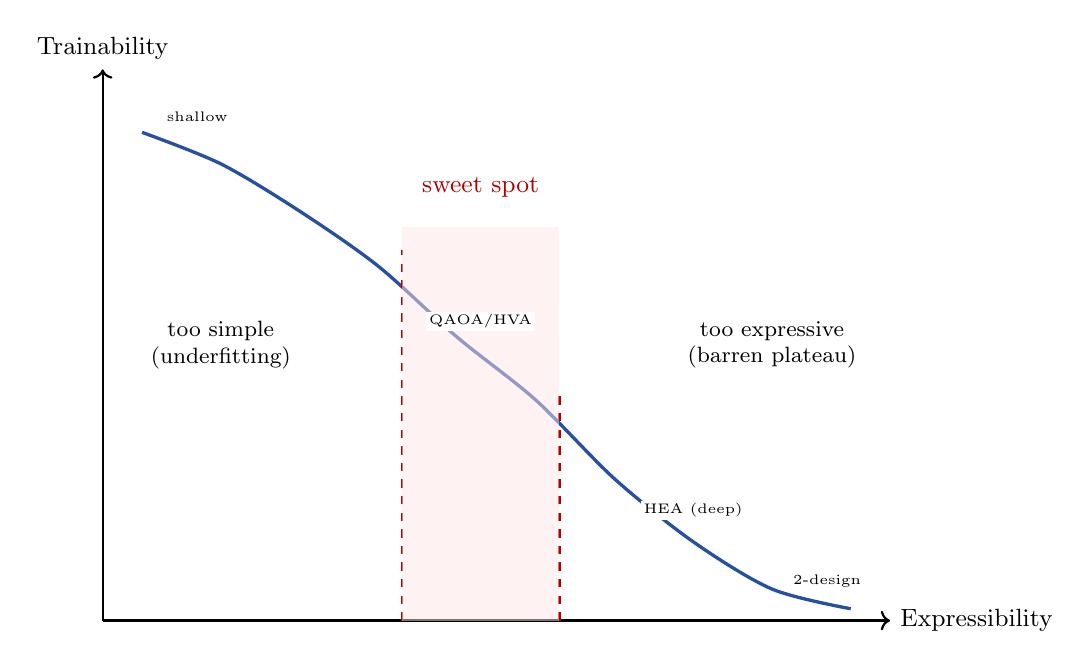
\begin{tikzpicture}[scale=1.0]
    % Axes
    \draw[->, thick] (0,0) -- (10,0) node[right, font=\small] {Expressibility};
    \draw[->, thick] (0,0) -- (0,7) node[above, font=\small] {Trainability};

    % Tradeoff curve
    \draw[very thick, circuitblue, smooth] plot coordinates {
        (0.5, 6.2) (1.5, 5.8) (2.5, 5.2) (3.5, 4.5) (4.5, 3.6)
        (5.5, 2.8) (6.5, 1.8) (7.5, 1.0) (8.5, 0.4) (9.5, 0.15)
    };

    % Labels for regions
    \node[font=\footnotesize, align=center] at (1.5, 3.5) {too simple\\(underfitting)};
    \node[font=\footnotesize, align=center] at (8.5, 3.5) {too expressive\\(barren plateau)};

    % Sweet spot
    \draw[thick, red!70!black, dashed] (3.8, 0) -- (3.8, 4.7);
    \draw[thick, red!70!black, dashed] (5.8, 0) -- (5.8, 2.9);
    \fill[red!10, opacity=0.5] (3.8, 0) rectangle (5.8, 5);
    \node[font=\small, red!70!black, align=center] at (4.8, 5.5) {sweet spot};

    % Ansatz labels
    \node[font=\tiny, fill=white, inner sep=1pt] at (1.2, 6.4) {shallow};
    \node[font=\tiny, fill=white, inner sep=1pt] at (4.8, 3.8) {QAOA/HVA};
    \node[font=\tiny, fill=white, inner sep=1pt] at (7.5, 1.4) {HEA (deep)};
    \node[font=\tiny, fill=white, inner sep=1pt] at (9.2, 0.5) {2-design};

\end{tikzpicture}
\end{center}

\begin{keypoint}
the sweet spot is problem-dependent. for a simple problem, a less expressive (more trainable) circuit suffices. for a complex problem, u need more expressiveness and must accept harder training. the art of QML circuit design is finding the right point on this curve for ur specific problem.
\end{keypoint}

%% ========================================================
\section{The Lie Algebra Perspective}
%% ========================================================

larocca, sauvage, nardo, coles, and cerezo developed a beautiful framework connecting trainability to the algebraic structure of the circuit.

\subsection{Dynamical Lie Algebra (DLA)}

\begin{definition}[Dynamical Lie Algebra]
given a parameterized circuit with generators $\{iH_1, iH_2, \ldots, iH_m\}$ (where $U_k(\theta_k) = e^{-i\theta_k H_k}$), the DLA is:
\begin{equation}
    \mathfrak{g} = \text{span}_{\mathbb{R}}\left\langle iH_1, \ldots, iH_m, [iH_j, iH_k], [[iH_j, iH_k], iH_l], \ldots \right\rangle
\end{equation}
the real vector space generated by the generators and all their nested commutators.
\end{definition}

the dimension $\text{dim}(\mathfrak{g})$ determines everything:
\begin{itemize}
    \item $\text{dim}(\mathfrak{g}) = 4^n - 1$ (maximal, $\mathfrak{su}(2^n)$): the circuit can reach any unitary. this is the 2-design regime. guaranteed barren plateau.
    \item $\text{dim}(\mathfrak{g}) \in O(\text{poly}(n))$: the circuit is restricted to a polynomial-dimensional subspace of unitaries. no barren plateau.
\end{itemize}

\begin{theorem}[Larocca et al. --- DLA Dimension Determines Trainability]
for a parameterized circuit with DLA $\mathfrak{g}$:
\begin{equation}
    \text{Var}[\partial_k C] \in \Theta\left(\frac{1}{\text{dim}(\mathfrak{g})}\right)
\end{equation}
\end{theorem}

this is incredibly clean. the gradient variance scales inversely with the DLA dimension. polynomial DLA = polynomial gradients = trainable. exponential DLA = exponential vanishing = barren plateau.

\subsection{DLA Dimensions of Common Ansatze}

\begin{center}
\renewcommand{\arraystretch}{1.4}
\begin{tabular}{|l|c|c|}
\hline
\textbf{Ansatz} & \textbf{dim($\mathfrak{g}$)} & \textbf{Barren Plateau?} \\
\hline
HEA (deep, all-to-all) & $4^n - 1$ & yes (exponential) \\
\hline
QAOA ($p$ layers) & $O(n)$ & no \\
\hline
HVA (1D Heisenberg) & $O(n^2)$ & no \\
\hline
particle-conserving & $\binom{n}{k}^2 - 1$ & depends on $k$ \\
\hline
matchgate circuits & $O(n^2)$ & no \\
\hline
single-qubit gates only & $3n$ & no \\
\hline
\end{tabular}
\end{center}

\begin{intuition}
the DLA perspective gives a simple recipe: before training a circuit, compute (or estimate) the dimension of its lie algebra. if its polynomial in $n$, ur safe. if its exponential, ur in trouble. this can often be done analytically for structured ansatze, or numerically for small instances.
\end{intuition}

%% ========================================================
\section{Gradient Variance vs Number of Qubits}
%% ========================================================

lets visualize the core phenomenon.

\subsection{Exponential Decay of Gradient Variance}

\begin{center}
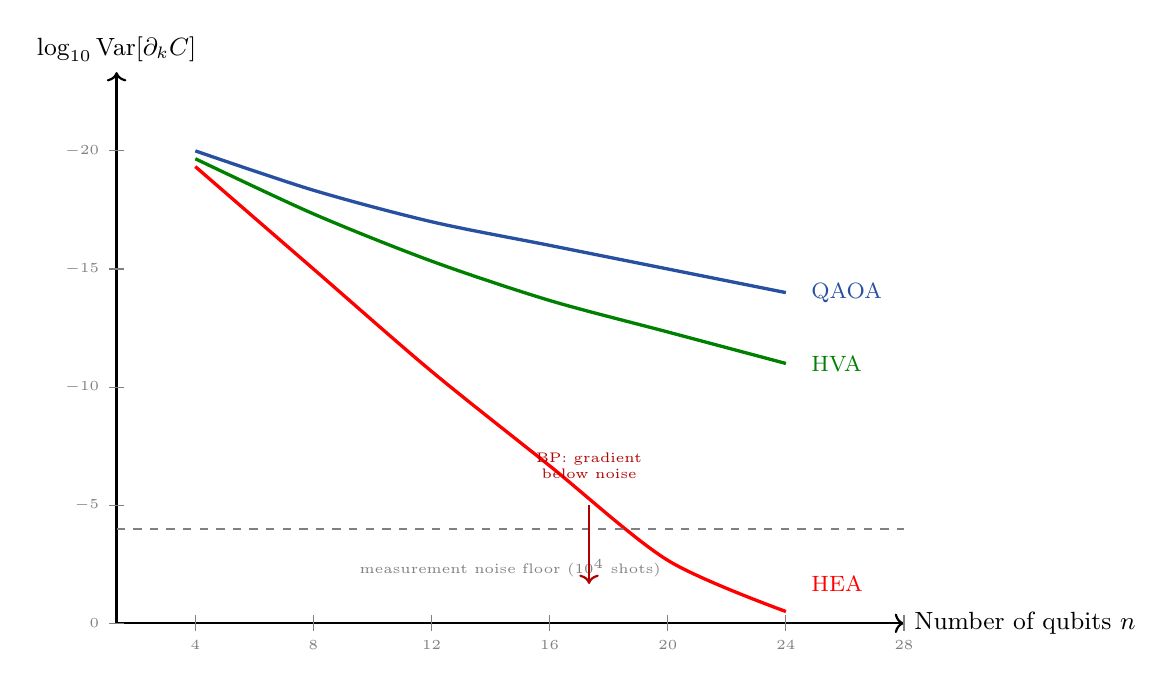
\begin{tikzpicture}[scale=1.0]
    % Axes
    \draw[->, thick] (0,0) -- (10,0) node[right, font=\small] {Number of qubits $n$};
    \draw[->, thick] (0,0) -- (0,7) node[above, font=\small, align=center] {$\log_{10}\text{Var}[\partial_k C]$};

    % Y-axis labels
    \foreach \y/\label in {0/$0$, 1.5/$-5$, 3/$-10$, 4.5/$-15$, 6/$-20$} {
        \draw[thin, gray] (0.1, \y) -- (-0.1, \y) node[left, font=\tiny] {\label};
    }

    % X-axis labels
    \foreach \x/\label in {1/4, 2.5/8, 4/12, 5.5/16, 7/20, 8.5/24, 10/28} {
        \draw[thin, gray] (\x, 0.1) -- (\x, -0.1) node[below, font=\tiny] {\label};
    }

    % HEA (exponential decay)
    \draw[very thick, red, smooth] plot coordinates {
        (1, 5.8) (2.5, 4.5) (4, 3.2) (5.5, 2.0) (7, 0.8) (8.5, 0.15)
    };
    \node[font=\footnotesize, red, right] at (8.7, 0.5) {HEA};

    % QAOA (polynomial decay)
    \draw[very thick, circuitblue, smooth] plot coordinates {
        (1, 6.0) (2.5, 5.5) (4, 5.1) (5.5, 4.8) (7, 4.5) (8.5, 4.2)
    };
    \node[font=\footnotesize, circuitblue, right] at (8.7, 4.2) {QAOA};

    % HVA (polynomial decay, slightly faster)
    \draw[very thick, green!50!black, smooth] plot coordinates {
        (1, 5.9) (2.5, 5.2) (4, 4.6) (5.5, 4.1) (7, 3.7) (8.5, 3.3)
    };
    \node[font=\footnotesize, green!50!black, right] at (8.7, 3.3) {HVA};

    % Measurement noise floor
    \draw[thick, dashed, gray] (0, 1.2) -- (10, 1.2);
    \node[font=\tiny, gray, align=center] at (5, 0.7) {measurement noise floor ($10^4$ shots)};

    % Arrow showing BP kicks in
    \draw[->, thick, red!70!black] (6, 1.5) -- (6, 0.5);
    \node[font=\tiny, red!70!black, align=center] at (6, 2.0) {BP: gradient\\below noise};

\end{tikzpicture}
\end{center}

the plot shows the key difference: HEA gradient variance decays exponentially (straight line on log scale), while QAOA and HVA decay polynomially (much slower). the horizontal dashed line represents the measurement noise floor --- below this, u cant distinguish the gradient from zero. for HEA, this happens around $n = 20$; for problem-inspired ansatze, the gradient stays well above the noise floor for much larger systems.

%% ========================================================
\section{Practical Guidelines for Circuit Design}
%% ========================================================

based on everything weve covered, here r concrete guidelines for designing trainable quantum circuits.

\subsection{The Checklist}

\begin{enumerate}[label=\textbf{G\arabic*.}]
    \item \textbf{use local cost functions}. decompose ur objective into a sum of terms, each acting on $O(1)$ qubits. avoid global observables like state fidelity unless absolutely necessary.

    \item \textbf{keep circuits shallow}. target depth $L \in O(\log n)$ to $O(\text{poly}(\log n))$. if u need more depth, use layer-wise training to get there incrementally.

    \item \textbf{prefer problem-inspired ansatze}. if ur problem has known structure (symmetries, locality, conservation laws), build them into the circuit. QAOA for optimization, HVA for physics, symmetry-preserving for chemistry.

    \item \textbf{initialize near identity}. set initial parameters close to zero so $U(\theta_0) \approx \mathbb{I}$. add small random perturbations $\sim \mathcal{N}(0, 0.01)$ to break symmetry.

    \item \textbf{limit entanglement growth}. dont use all-to-all connectivity unless needed. nearest-neighbor entangling gates create less entanglement per layer and delay the onset of BPs.

    \item \textbf{check the DLA dimension}. if u can compute or estimate $\text{dim}(\mathfrak{g})$ for ur ansatz, do it. polynomial dimension = safe. exponential = redesign.

    \item \textbf{account for noise}. circuit depth is bounded by $O(1/p)$ where $p$ is the gate error rate. dont design circuits deeper than ur hardware can support.

    \item \textbf{monitor gradient norms during training}. if gradients are shrinking as u scale up qubits, thats a red flag. plot $\text{Var}[\partial_k C]$ vs $n$ to check for exponential decay.

    \item \textbf{use parameter correlations wisely}. sharing parameters across layers (like in QAOA) reduces the effective parameter space and can improve trainability. but it also limits expressiveness.

    \item \textbf{consider alternatives to gradient descent}. evolutionary strategies, bayesian optimization, and model-based methods dont rely on gradient information and can sometimes navigate barren plateaus. but they have their own scaling issues.
\end{enumerate}

\subsection{Decision Flowchart}

\begin{center}
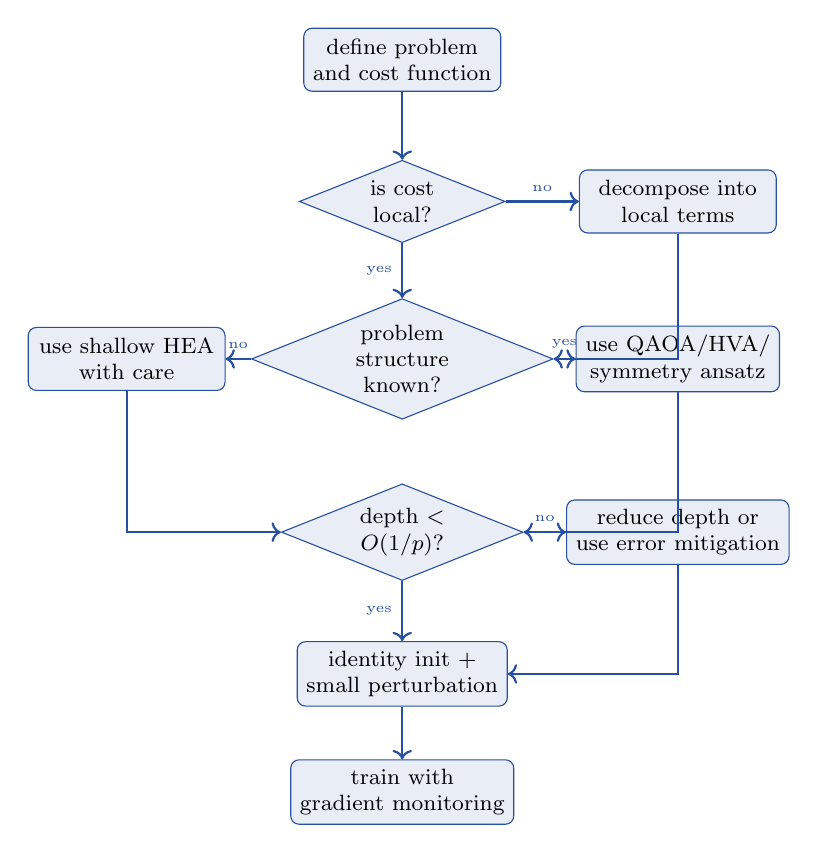
\begin{tikzpicture}[
    decision/.style={diamond, draw=circuitblue, fill=circuitblue!10,
        aspect=2.5, inner sep=2pt, font=\footnotesize, align=center},
    process/.style={rectangle, draw=circuitblue, fill=circuitblue!10,
        rounded corners=3pt, minimum width=2.5cm, minimum height=0.8cm,
        font=\footnotesize, align=center},
    arrow/.style={->, thick, circuitblue},
    yesno/.style={font=\tiny, circuitblue}
]

\node[process] (start) at (0, 0) {define problem\\and cost function};
\node[decision] (q1) at (0, -1.8) {is cost\\local?};
\node[process] (fix1) at (3.5, -1.8) {decompose into\\local terms};
\node[decision] (q2) at (0, -3.8) {problem\\structure\\known?};
\node[process] (use_pi) at (3.5, -3.8) {use QAOA/HVA/\\symmetry ansatz};
\node[process] (use_hea) at (-3.5, -3.8) {use shallow HEA\\with care};
\node[decision] (q3) at (0, -6.0) {depth $<$\\$O(1/p)$?};
\node[process] (fix3) at (3.5, -6.0) {reduce depth or\\use error mitigation};
\node[process] (init) at (0, -7.8) {identity init +\\small perturbation};
\node[process] (train) at (0, -9.3) {train with\\gradient monitoring};

\draw[arrow] (start) -- (q1);
\draw[arrow] (q1) -- node[yesno, left] {yes} (q2);
\draw[arrow] (q1) -- node[yesno, above] {no} (fix1);
\draw[arrow] (fix1) |- (q2);
\draw[arrow] (q2) -- node[yesno, above] {yes} (use_pi);
\draw[arrow] (q2) -- node[yesno, above] {no} (use_hea);
\draw[arrow] (use_pi) |- (q3);
\draw[arrow] (use_hea) |- (q3);
\draw[arrow] (q3) -- node[yesno, left] {yes} (init);
\draw[arrow] (q3) -- node[yesno, above] {no} (fix3);
\draw[arrow] (fix3) |- (init);
\draw[arrow] (init) -- (train);

\end{tikzpicture}
\end{center}

%% ========================================================
\section{Advanced Topics}
%% ========================================================

\subsection{Overparameterization and Lazy Training}

larocca et al. also showed an interesting connection to classical deep learning: when a PQC has many more parameters than needed (overparameterized), it can enter a ``lazy training'' regime where the parameters barely move from initialization. this avoids BPs but at the cost of the model essentially being linear around the initial point.

\begin{equation}
    f(x; \theta) \approx f(x; \theta_0) + \nabla_\theta f(x; \theta_0)^T (\theta - \theta_0)
\end{equation}

this is the quantum analog of the neural tangent kernel (NTK) regime. the model is effectively a kernel method with kernel:
\begin{equation}
    k_{\text{NTK}}(x, x') = \nabla_\theta f(x; \theta_0)^T \nabla_\theta f(x'; \theta_0)
\end{equation}

\subsection{Quantum Natural Gradient}

the quantum natural gradient (stokes et al. 2020) uses the fubini-study metric to define a geometry-aware gradient:
\begin{equation}
    \theta_{t+1} = \theta_t - \eta \, F^{-1}(\theta_t) \nabla_\theta C(\theta_t)
\end{equation}
where $F$ is the quantum fisher information matrix:
\begin{equation}
    F_{ij} = \text{Re}\left[\braket{\partial_i \psi | \partial_j \psi} - \braket{\partial_i \psi | \psi}\braket{\psi | \partial_j \psi}\right]
\end{equation}

this can help with barren plateaus bcs it rescales the gradient by the curvature of the parameter space. in flat regions, $F$ is small and $F^{-1}$ amplifies the gradient. however, computing $F$ requires $O(p^2)$ circuit evaluations for $p$ parameters, which is expensive.

\begin{keypoint}
quantum natural gradient doesnt \emph{solve} barren plateaus --- the gradient is still exponentially small. but $F^{-1}$ can partially compensate, effectively converting an exponentially small gradient into a polynomially small effective gradient in some cases. its a mitigation, not a cure.
\end{keypoint}

\subsection{Error Mitigation and Trainability}

error mitigation techniques (zero-noise extrapolation, probabilistic error cancellation) can partially address noise-induced BPs by reducing the effective noise rate. however, they come with their own overhead:
\begin{equation}
    \text{cost of mitigation} \sim O\left(\frac{1}{q^{2L}}\right)
\end{equation}
where $q = 1 - p$. this is exactly the same exponential factor that causes the noise-induced BP, so error mitigation and noise-induced BPs have the same scaling --- u cant fully mitigate ur way out of a noise-induced BP.

%% ========================================================
\section{Open Questions}
%% ========================================================

barren plateaus r still an active research area. here r key open questions:

\begin{enumerate}[label=\arabic*.]
    \item \textbf{tight bounds}: the current bounds on gradient variance r often loose. can we get tight (matching upper and lower) bounds for specific architectures?

    \item \textbf{higher-order methods}: can second-order optimization (hessian-based) escape barren plateaus? the hessian itself might vanish exponentially, but theres ongoing work here

    \item \textbf{quantum advantage despite BPs}: r there problems where the barren plateau threshold is higher for quantum models than for equivalent classical models? this would still give a relative advantage

    \item \textbf{adaptive circuits}: circuits that change structure during training (adding/removing gates) might navigate the expressibility-trainability tradeoff dynamically. ADAPT-VQE is one example

    \item \textbf{measurement-based strategies}: can mid-circuit measurements and classical feedforward help avoid BPs? early evidence suggests yes, but the theory is incomplete

    \item \textbf{non-gradient methods at scale}: evolutionary strategies, reinforcement learning for parameter optimization, random search --- can these scale better than gradient descent in BP regimes?
\end{enumerate}

%% ========================================================
\section{Summary}
%% ========================================================

this was a dense lecture bcs barren plateaus r the make-or-break issue for variational QML. lets consolidate:

\begin{enumerate}[label=\arabic*.]
    \item \textbf{barren plateaus} = gradient variance vanishes exponentially with system size. this makes optimization impossible with polynomial resources.

    \item \textbf{four mechanisms}: expressibility (mcclean 2018), global cost functions (cerezo 2021), noise (wang 2021), entanglement (marrero 2021). they can act independently.

    \item \textbf{mcclean et al.}: random circuits that form 2-designs have $\text{Var}[\partial_k C] \in O(2^{-n})$. this is the foundational result.

    \item \textbf{cerezo et al.}: local cost functions save u --- gradient variance depends on depth $L$, not width $n$. use local costs whenever possible.

    \item \textbf{noise-induced BPs}: hardware noise independently kills trainability for circuits deeper than $O(1/p)$. this is a hard physical limit.

    \item \textbf{entanglement}: too much entanglement scrambles gradient information. control entanglement growth through circuit design.

    \item \textbf{kernel concentration}: barren plateaus in variational models correspond to kernel concentration in kernel models. same root cause (2-design convergence), same cure (restrict expressibility).

    \item \textbf{DLA dimension}: the dimension of the dynamical lie algebra determines trainability. polynomial DLA = trainable, exponential DLA = barren plateau. this is the cleanest characterization we have.

    \item \textbf{mitigation strategies}: local costs, shallow circuits, layer-wise training, identity initialization, problem-inspired ansatze. use all of them.

    \item \textbf{the fundamental tradeoff}: expressibility vs trainability. u cant have both. the art is finding the sweet spot for ur specific problem.
\end{enumerate}

\begin{keypoint}
if u remember one thing from this lecture: \textbf{more expressive is not better}. the best quantum models r not the most general ones --- they r the ones that r just expressive enough for the task while remaining trainable. this principle should guide every circuit design decision u make.
\end{keypoint}

next lecture well look at concrete strategies for benchmarking and evaluating quantum models, including proper comparison with classical baselines.

\end{document}
